\documentclass[11pt]{scrartcl}
\usepackage{graphicx}

% Configure listings for MATLAB code
\usepackage{color}
\usepackage{listings}

\definecolor{dkgreen}{rgb}{0,0.6,0}
\definecolor{gray}{rgb}{0.5,0.5,0.5}

\lstset{language=Matlab,
   keywords={break,case,catch,continue,else,elseif,end,for,function,
      global,if,otherwise,persistent,return,switch,try,while},
   basicstyle=\ttfamily\scriptsize,
   keywordstyle=\color{blue},
   commentstyle=\color{gray},
   stringstyle=\color{dkgreen},
   numbers=left,
   numberstyle=\tiny\color{gray},
   stepnumber=1,
   numbersep=10pt,
   backgroundcolor=\color{white},
   tabsize=4,
   showspaces=false,
   showstringspaces=false}


\begin{document}

\title{Final Project Report}
\subtitle{18-758 Wireless Communications}
\author{Michael Nye (mnye)}
\date{}
\maketitle



\section*{System Design}

\subsection*{Modulation}

For my final project, I designed a system fairly similar to what was shown in
lectures. For coding, I used a rate-1/2 convolution code with 4 states. After
codig, the symbol bits are interleaved by a factor of 132 (chosen to be a large
integral factor of my packet size). Again, testing of my system has demonstrated
that this coding scheme sufficiently decouples error events and allows robust
correction given my channel.

I use an 8-PSK modulation scheme. My choice of eight points was motivated by
empirical measurements of the channel; I used the highest order constellation
I could support without the noise causing symbol errors. I then used a hamming
window pulse. The hamming window was chosen as it has better bandwidth
properties than other FIR windows, but was easier to implement than
a multisymbol pulse such as a raised cosine rolloff pulse. Testing showed that
this pulse was sufficient to meet the project specifications.

Finally, I prepend my message with a single pilot sequence to facilitate
equalization and timing synchronization. The sequence is created by generating
a bit sequence. This sequence is a De Bruijn sequence, which creates a large
variety in symbol ordering to create a unique sequence. This sequence is then
modulated using a wide BPSK for easy detection.

Constant factors were chosen to be as large as possible while still meeting
channel requirements and message size. Since I was fixed to rate-1/2 coding and
3 bits per symbol, this meant to fit my entire message (3036 pixels) in the
allowed space, I was able to use at most 4 samples per symbol. I then expanded
my pilot sequence to fill most of the remaining space.


\subsection*{Demodulation}

My demodulator largely follows the reverse of my modulator. First off, I perform
carrier recovery. To do so, I compute a DTFT on my received signal over a range
of only low frequencies. I find the maximum amplitude frequency, and then divide
by a complex sinusoid of the same frequency.

This is followed by timing recovery and equalization. I find the correlation
between my pilot signal and the recovered signal. The maximum lag is the start
of my pilot sequence. I can then extract the pilot sequence, and detect the
pilot symbols. The channel equalization constant is then found by comparing the
detected symbols to the known pilot symbols. Finally, the received signal is
divided by this same factor to equalize.

At this point, I can window out only my message. I match filter the message,
then sampling the result and perform hard detection of the coded bits. After
deinterleaving these detected bits, I find the minimum error path through my
coding trellis to correct any bit errors in the coded bits. Finally, the
corrected coded bits are decoded into my message bits and returned.




\section*{Analysis}

My system largely follows the principles demonstrated in lectures. There are
three main differences I chose to make to simplify the system.

The first difference was my choice of pilot. I chose to use the same pilot
message for carrier recovery, timing recovery and equalization. My testing found
that this didn't cause any degradation of performance, and allowed me to
minimize the size of my header.

The second difference was my choice of window. While raised cosine rolloff
windows are clearly superior to hamming windows in terms of bandwidth
properties, I found it difficult to correctly design the window to prevent ISI.
A hamming window was much simpler to implement and performed admirably for my
purposes.

The final difference was in how I performed carrier recovery. While we were
encouraged to use a BPSK pilot sequence, I found this didn't provide sufficient
resolution to find the carrier offset frequency. I instead just used the entire
received signal, and bandlimited the region I search for the peak in the
frequency domain. This proved surprisingly effective, and so I stuck with it.

The other difficulties I ran into were simply implementation details. Until this
project, I had never used the MATLAB \verb|'| operator to transpose complex
data.  I learned that this was a hermitian transpose, but it lingered in dark
corners of my code base, and took quite a while to track down the errors. I also
spent a lot of time determining exact offsets for my sampling times. This
complexity was simply an artifact of using convolution with MATLAB vectors, and
the resulting offsets it introduces into my data.



\section*{MATLAB Implementation}

On the following pages, I have attached the code used to implement my
communications system. There are three files. The first is {\tt constants.m},
and contains just a set of constants referenced in my modulator and demodulator.
The second is {\tt generate transmit signal.m}, and contains a function that
given a bit sequence will return a transmit signal. Finally, {\tt
decode received signal.m} takes in a received signal and performs recovers the
original message in the transmit signal.

\pagebreak
\lstinputlisting{../constants.m}

\pagebreak
\lstinputlisting{../create_transmit_signal.m}

\pagebreak
\lstinputlisting{../decode_received_signal.m}



\pagebreak
\section*{Operational Figures}

On the following pages, I have attached sample figures demonstrating my the
functioning of my system. I have shown a higher-than-average noise sample
demonstrating that even under harder transmit criteria, I receive less than
a .3\% error rate.

\begin{figure}[h]
    \centering
    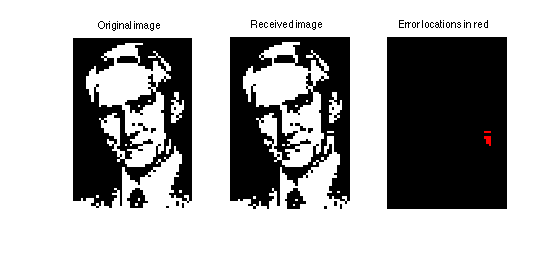
\includegraphics[width=1.0\textwidth]{figures/receivedimage.png}
    \caption{Comparison of transmitted and received images}
\end{figure}

\begin{figure}
    \centering
    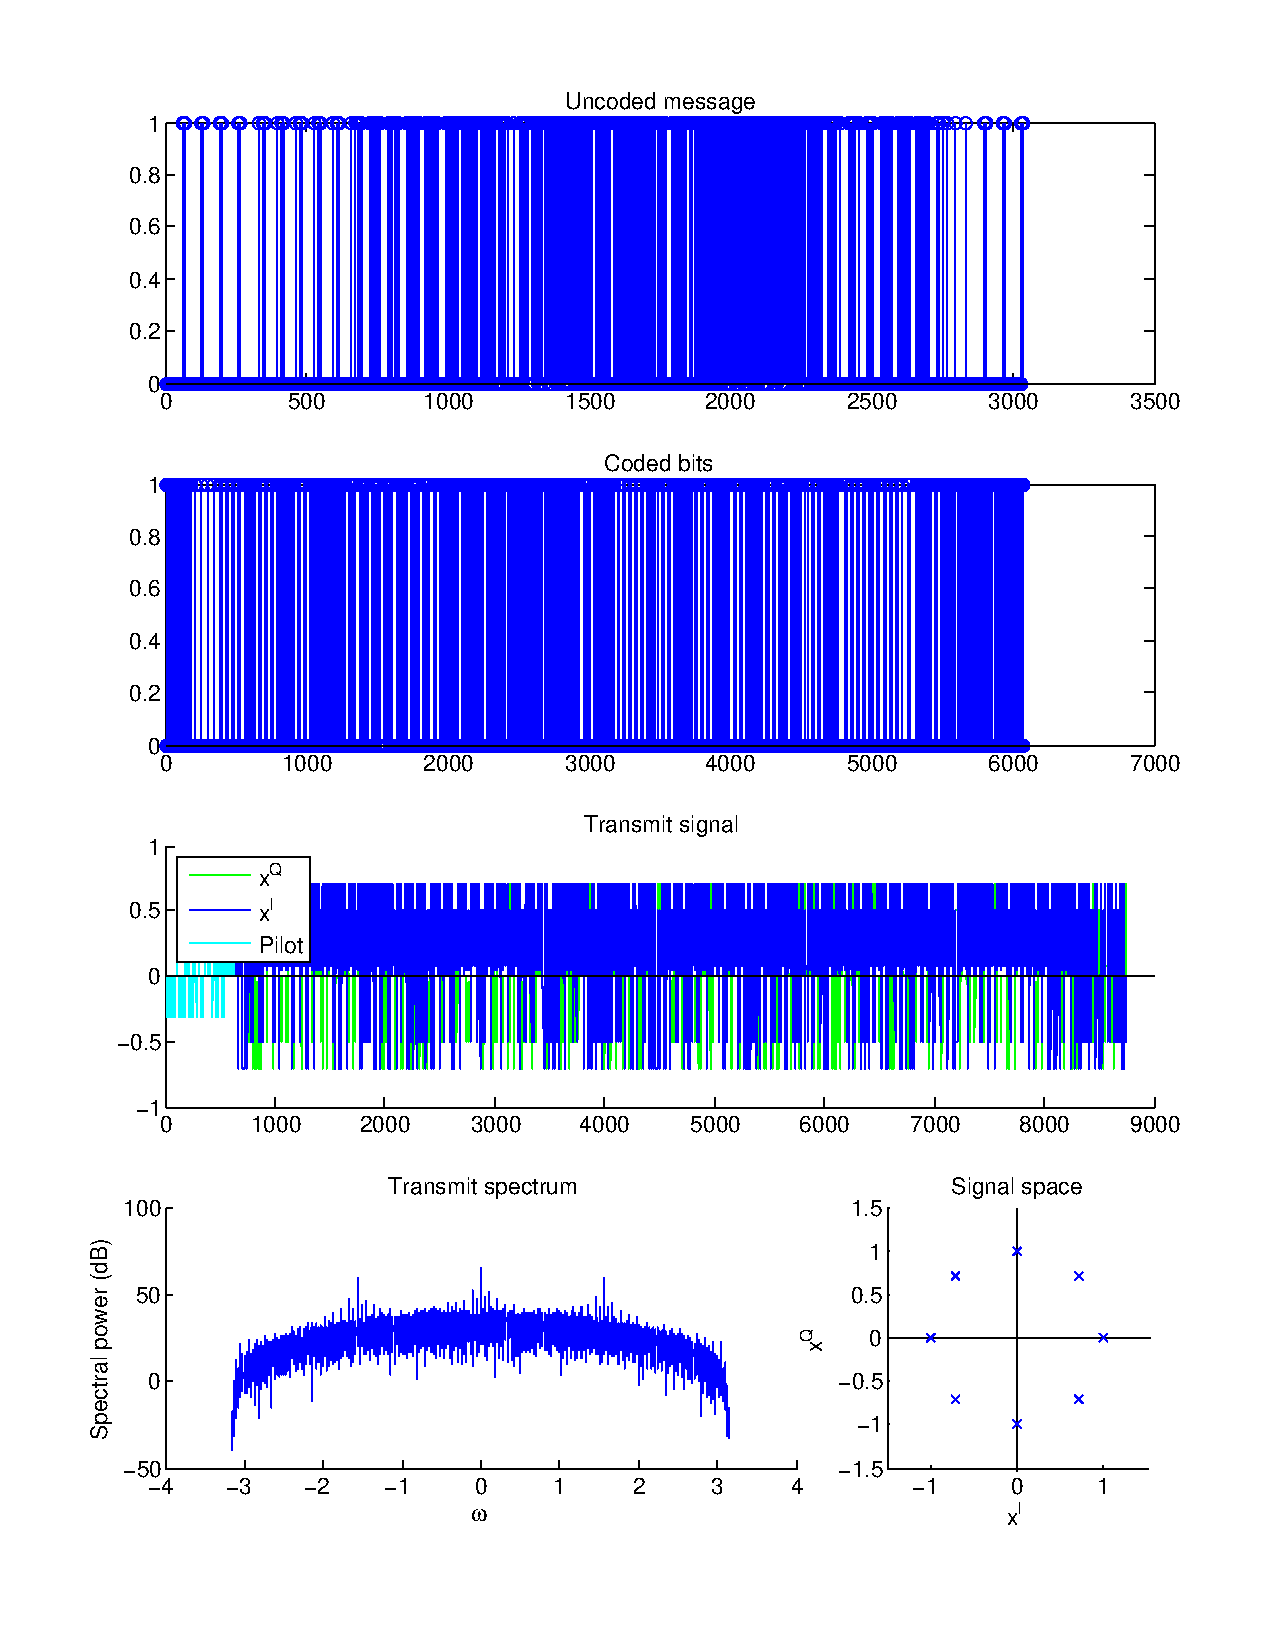
\includegraphics[width=1.0\textwidth]{figures/transmit.pdf}
    \caption{Generated transmit signal}
\end{figure}

\begin{figure}
    \centering
    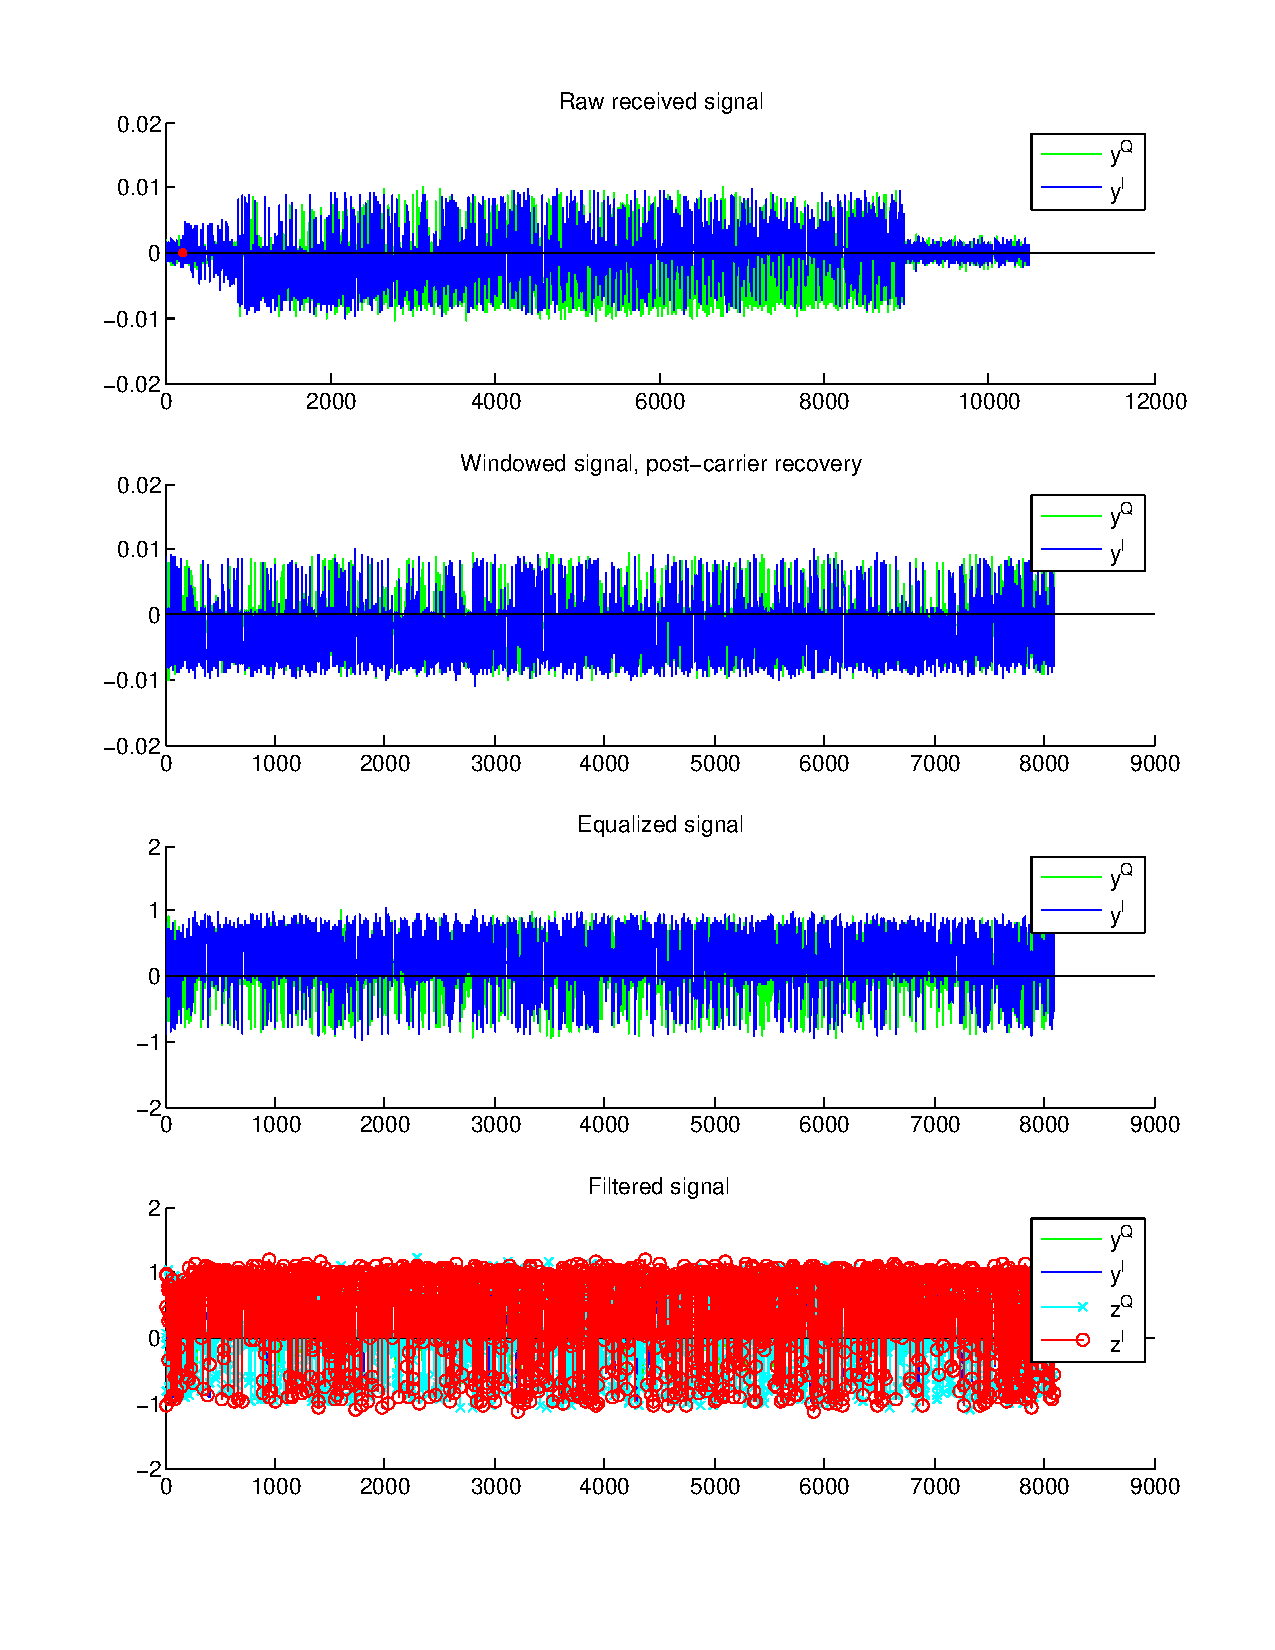
\includegraphics[width=1.0\textwidth]{figures/receivedsignal.pdf}
    \caption{Signal received from radio, and various processing}
\end{figure}

\begin{figure}
    \centering
    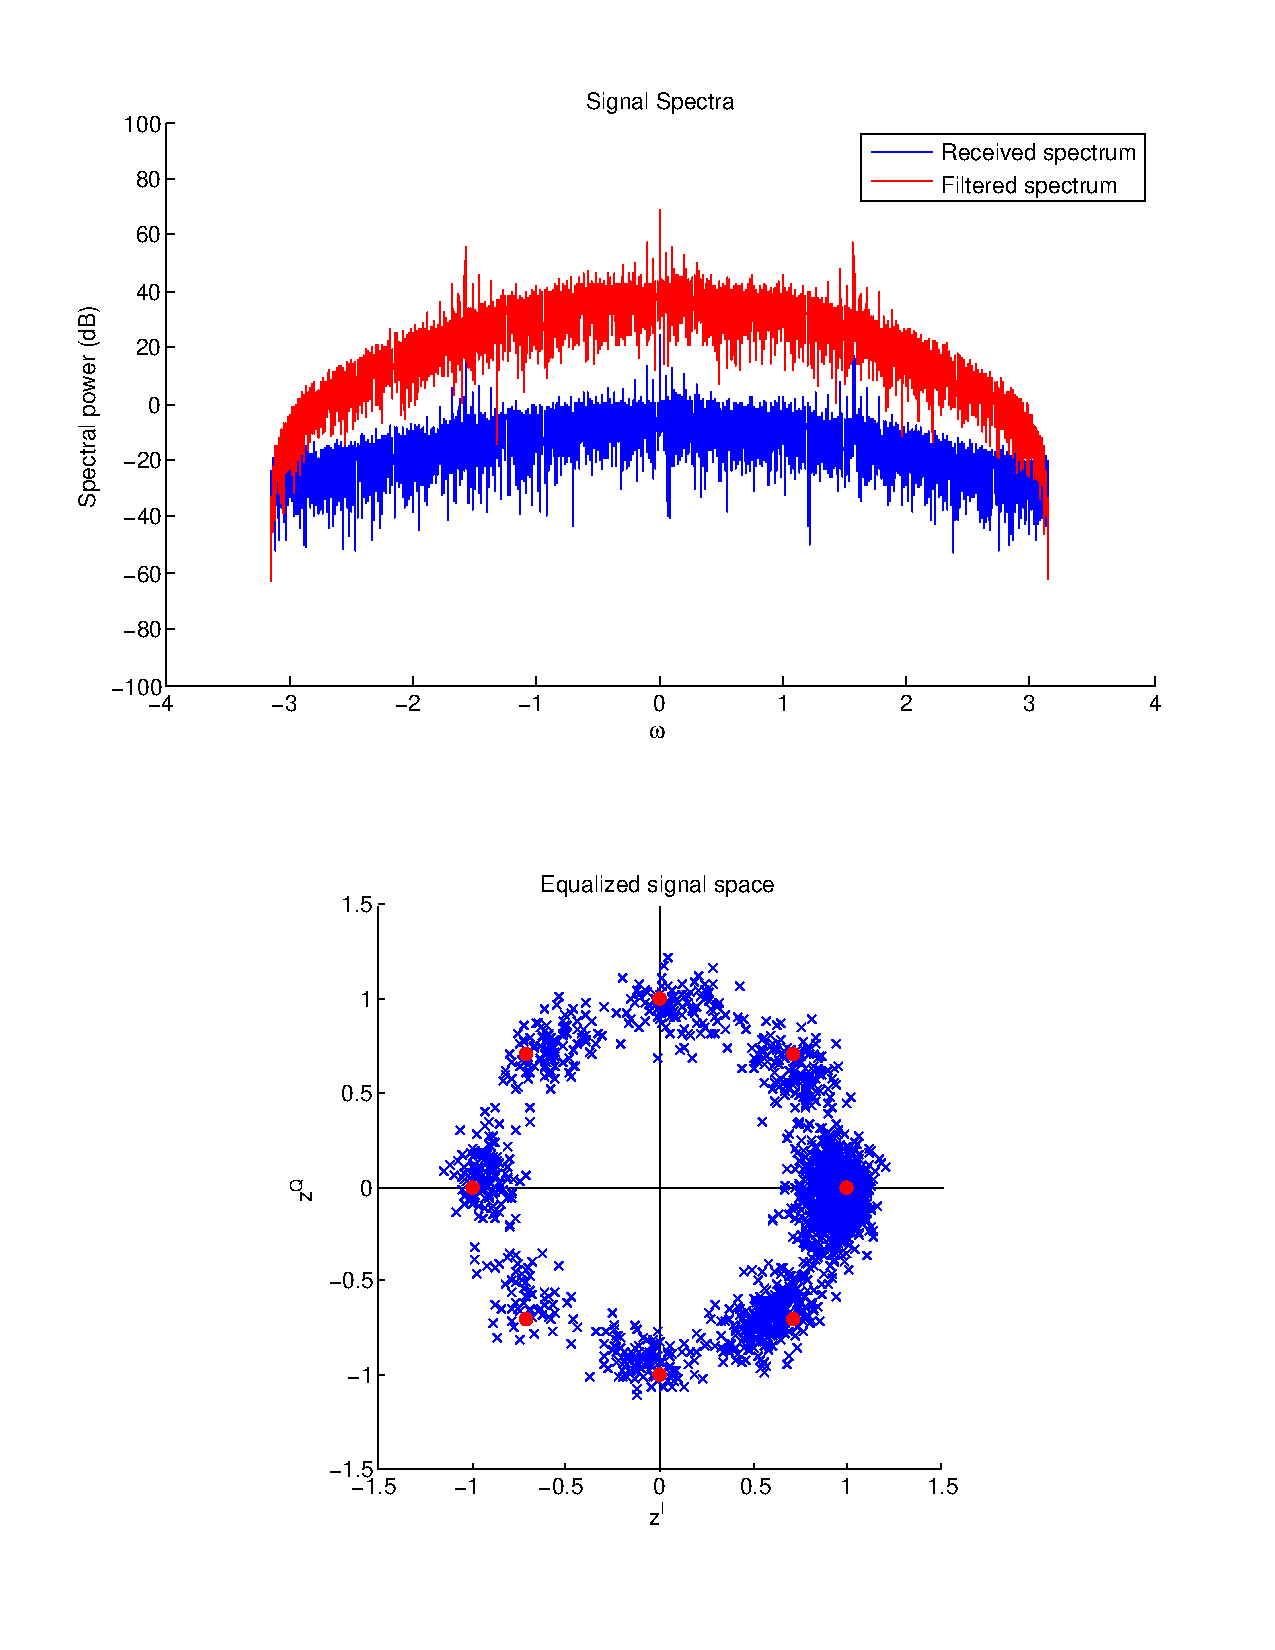
\includegraphics[width=1.0\textwidth]{figures/receivedspectra.pdf}
    \caption{Received signal spectra and signal space}
\end{figure}

\begin{figure}
    \centering
    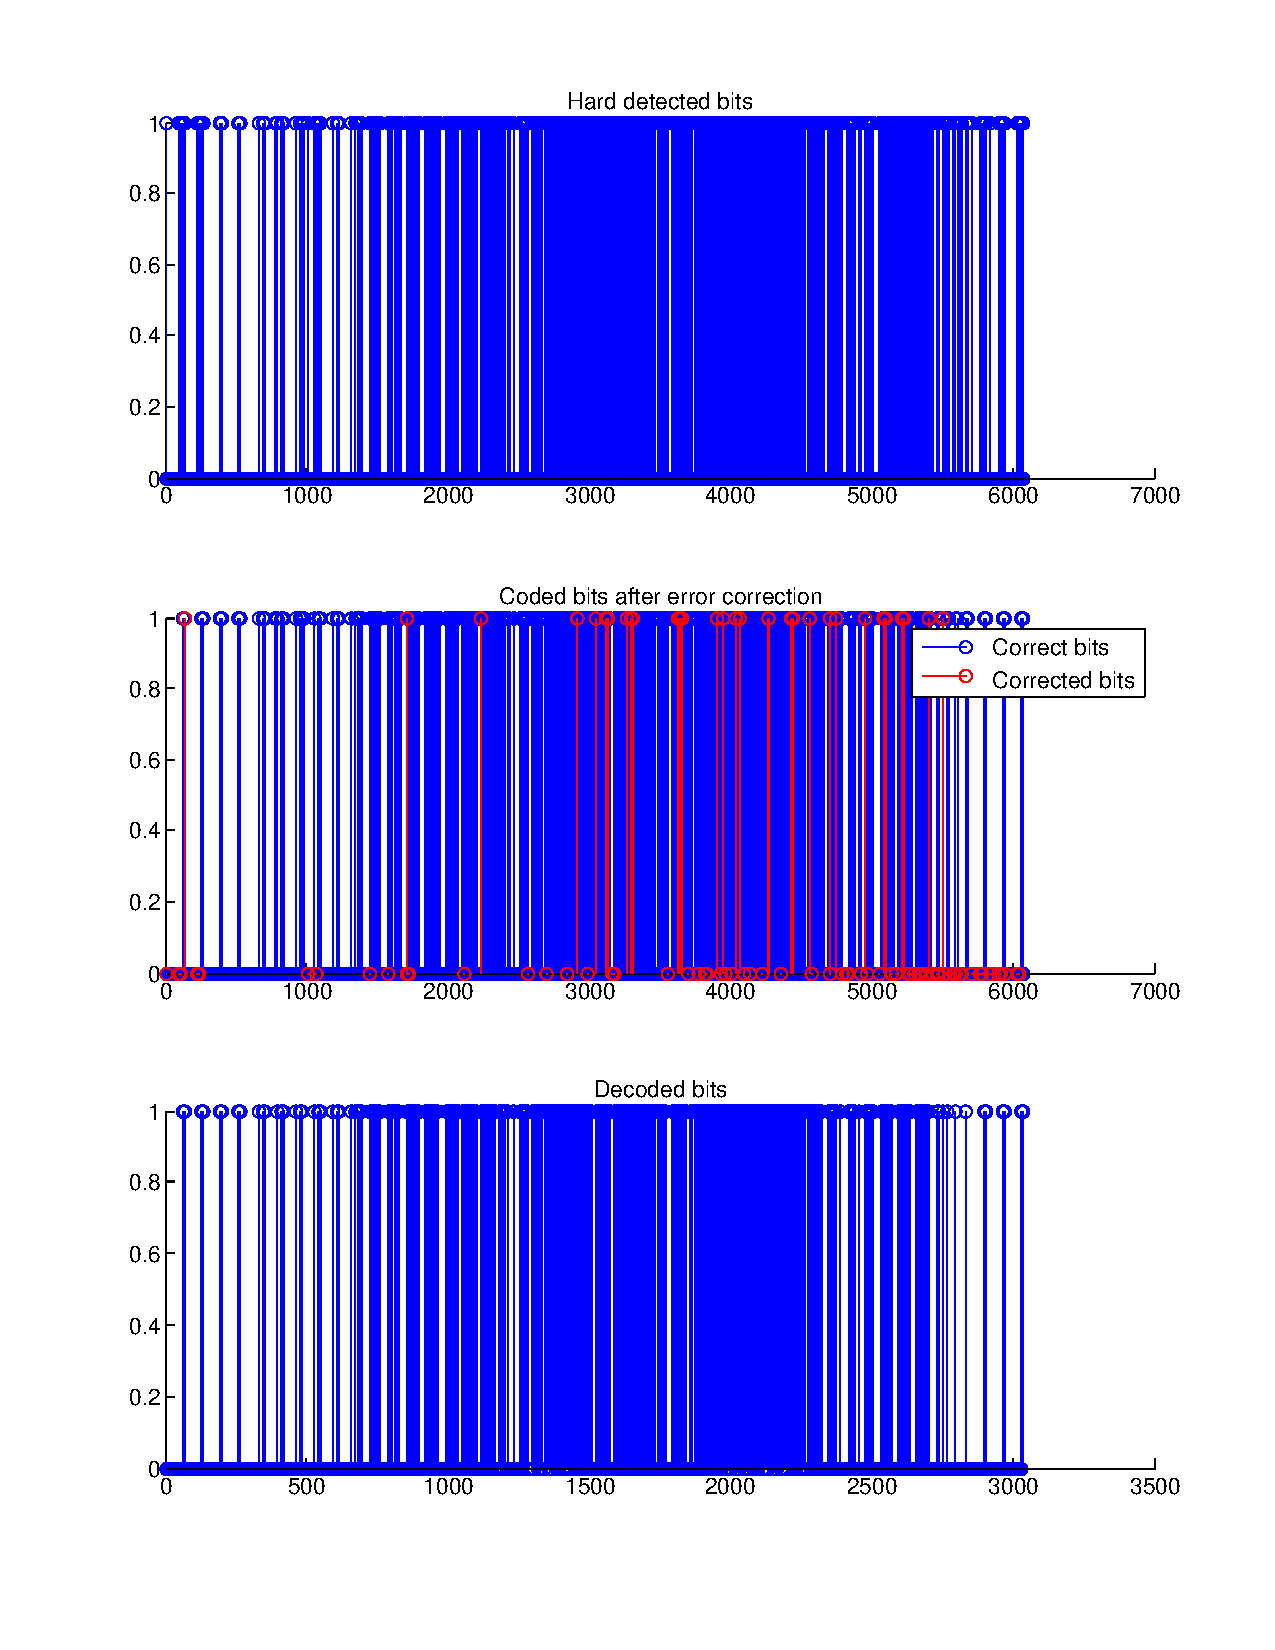
\includegraphics[width=1.0\textwidth]{figures/receivedbits.pdf}
    \caption{Received signal bits, and decoding}
\end{figure}



\end{document}
